With the advent of deep learning, the development of machine learning centered on neural networks has reached its heyday.
While a neural network called a multilayer perceptron performed an approximation of an arbitrary function by combining nonlinear transformation with one hidden layer, in Deep Neural Network(DNN), the expressive ability of the neural network is dramatically improved by increasing the number of hidden layers and performing an iterative nonlinear transformation.
In the massive image recognition competition ILSVRC ~\cite{bib:deng2009imagenet}, as shown in Fig.1, since the initial DNN AlexNet ~\cite{bib:alexnet-krizhevsky-nips2012} was proposed, we have achieved logarithmic accuracy improvement every year.
This makes it possible to approximate complex functions with the number of parameters that can be learned, and neural networks are expected to be applied to real problems. However, training data in proportion to the number of parameters are required to learn the latest neural network where hundreds of millions of parameters are used, and a huge amount of computing resources and time are required.
Furthermore, as can be seen from the change by year for the scale of the network model that won the ILSVRC in Fig.2, the size of the neural network is increasing exponentially, and problems due to the increase in the number of training data are expected to become more serious.


In this research, in order to tackle this problem, we propose a method to reduce training data while maintaining DNN accuracy. Focus on differences in importance in training data as a basic idea of the proposed method, and we will improve the efficiency of learning by performing neural network learning only with training data of high importance. In order to realize this, we focus on the role of support vectors in Support Vector Machine (SVM) ~\cite{bib:Support-Vector-Networks}. A support vector refers to a group of data used to define boundary hyperplanes in spatial separation of SVM. Therefore, the support vector has a feature located at the outermost part of the training data of the same class and is expected to play an essential role in the learning of neural networks. While existing research on training data reduction based on support vectors has provided initial results for MNIST, which is a handwritten digit recognition data set, it does not clarify the learnability for more complicated problems. In this study, we aim to clarify the effect of support vectors in DNN learning using ResNet ~\cite{bib:Deep-Residual-Learning-for-Image-Recognition} which is one of the newest neural networks and CIFAR-10 which is a data set for image classification.

\begin{figure}[t]
  \begin{minipage}{0.49\hsize}
\begin{center}
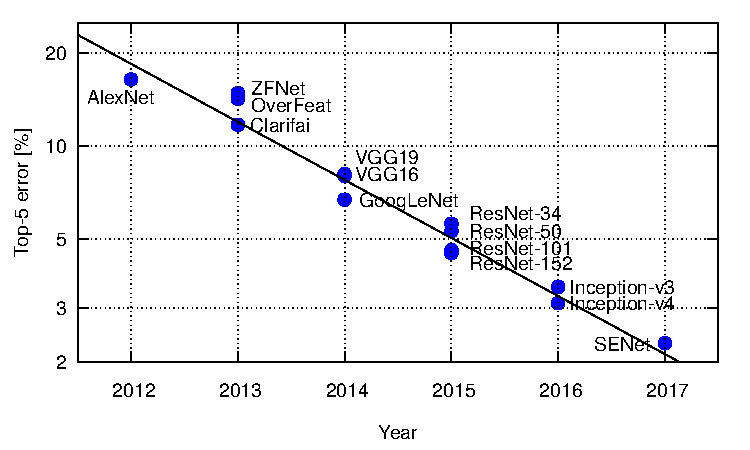
\includegraphics[width=\linewidth]{fig/y_o2.pdf}
\end{center}
\caption{Yearly error transition for ImageNet.}
\vspace*{-3pt}
%{\hfill\footnotesize Note how the caption is centered in the column.\hfill}
\end{minipage}
\begin{minipage}{0.49\hsize}
\begin{center}
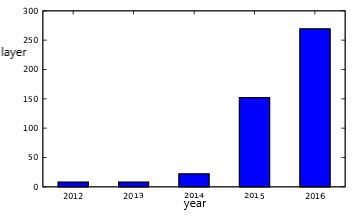
\includegraphics[width=\linewidth]{fig/fig2.png}
\end{center}
\caption{A scale change according to the year of ILSVRC championship model}
\vspace*{-3pt}
        %{\hfill\footnotesize Note how the caption is centered in the column.\hfill}
        \end{minipage}
\end{figure}


The composition of this paper is as follows. Section 2 explains the concepts of machine learning and deep learning, and the basics of neural networks and SVM used in this research.
Next, Section 3 explains the training data reduction method using support vectors, and verifies the effects of support vectors in neural network learning visually by performing preliminary experiments on multiple two-dimensional data. Section 4 shows the results of evaluation experiments using the latest neural network ResNet and the image data set CIFAR-10 and discusses the issues. Section 5 concludes with the conclusions.
